\documentclass{beamer}
\usepackage{beamerthemeCambridgeUS}
\usepackage{color}  % for \textcolor{red}{blah}
\usepackage{graphicx}
\usepackage{subfigure}
\usepackage{multicol}
\usepackage{verbatim} % for \begin{comment}
\usepackage{lipsum}


\newcommand\Fontvi{\fontsize{6}{7.2}\selectfont}


\newenvironment{packed_enum}{
\begin{enumerate}
  \setlength{\itemsep}{1pt}
  \setlength{\parskip}{0pt}
  \setlength{\parsep}{0pt}
}{\end{enumerate}}

\newenvironment{packed_item}{
\begin{itemize}
  \setlength{\itemsep}{1pt}
  \setlength{\parskip}{0pt}
  \setlength{\parsep}{0pt}
}{\end{itemize}}

\usetheme{CambridgeUS}

\title{Discrete Mathematics}
\author[Geoffrey Buhl]{Geoffrey Buhl \\ \texttt{geoffrey.buhl@csuci.edu}}
\institute[CSUCI]{California State University Channel Islands}
\date{\today}

\def \vec{{\rm vec}}
\newtheorem{conjecture}[theorem]{Conjecture}
\newtheorem{explanation}[theorem]{Explanation}


\begin{document}

%\frame{\titlepage}

%\section[Outline]{}
%\frame{\tableofcontents}

\section{Week 8 Class 2}


\frame
{
  \frametitle{Graph Theory Introduction}

Chapter 3 is an introduction to the mathematical objects graphs, which are a set up objects called vertices and a set of connections between these objects called edges.

\vfill
Class Session Goals:
\begin{packed_enum}
\item Become familiar graphs and basic graph theory definitions.
\item Construct some graphs and used these graphs to better understand the basic definitions.
\end{packed_enum}
\vfill
}




\frame
{
  \frametitle{Some application of graph theory}

Airline Scheduling - Flow problems \vfill
Directions in a map - Shortest path algorithms\vfill
Solving Sudoku's puzzles - Graph coloring algorithms\vfill
Search Engine Algorithms - PageRank algorithm\vfill
Social Media Marketing - Community detection via hierarchical clustering algorithms \vfill
Radio Frequency Allocation - Vertex coloring problem \vfill
}

\frame
{
  \frametitle{Frequency Allocation}

\begin{center}
 \begin{tabular}{c|c|c|c|c|c|c} 
 \hline
  & 1	 & 2 & 3 & 4 & 5 & 6 \\
 \hline
 1 & - & 85 & 175 &200 & 50 & 100 \\ 
 \hline
 2 &  85 & - & 125 & 175 & 100 & 160 \\ 
 \hline
 3 & 175 & 125 & - &100 & 200 & 250 \\ 
 \hline
 4 & 200 & 175 & 100 & - & 210 & 220 \\ 
 \hline
 5 &  50 & 100 & 200 & 210 & - & 100 \\  
 \hline
  6&  100 & 160 & 250 & 220 & 100 & - \\ 
 \hline
\end{tabular}
\end{center}

{\bf Step 1}:  For each station, 1 through 6, draw a line between the stations if the distance between the two is 150 or less.\\
{\bf Step 2}:  Determine the minimum numbers of colors need to color the vertices, so that adjacent vertices have different colors.

}


\frame
{
  \frametitle{Frequency Allocation Activity}


\begin{figure}[htp]
  \begin{center}
    \subfigure{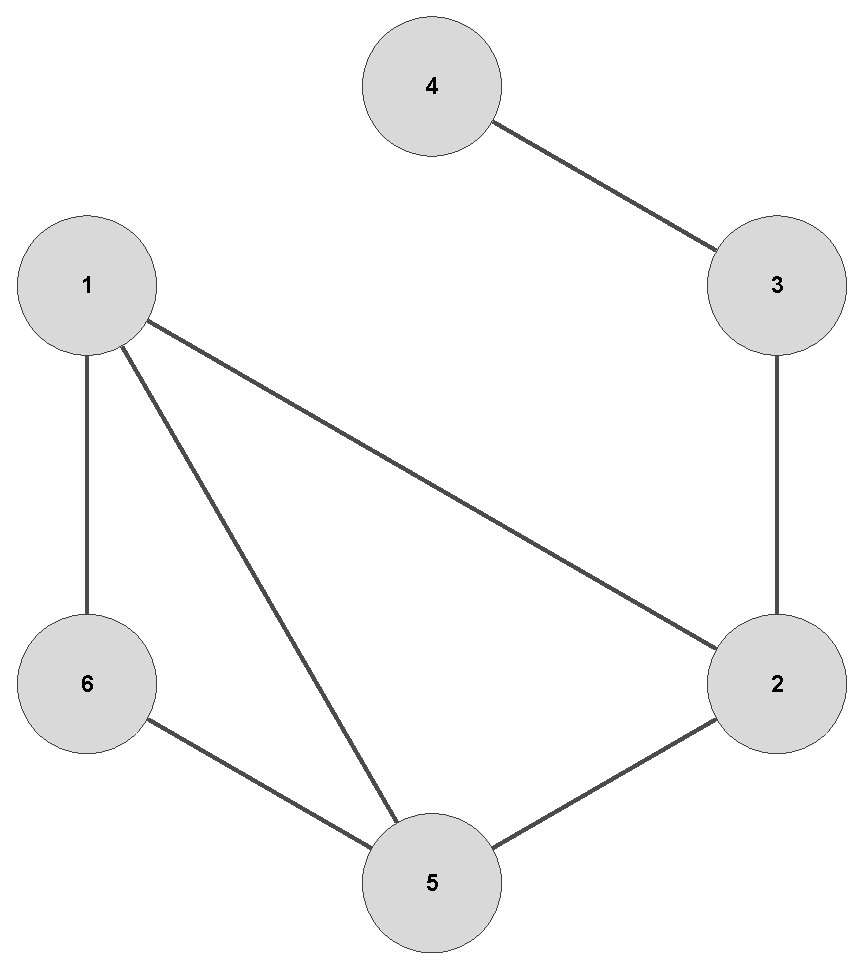
\includegraphics[scale=.4]{RFallocation2}}
  \end{center}
\end{figure}



}


\frame
{
  \frametitle{Frequency Allocation Activity}


\begin{figure}[htp]
  \begin{center}
    \subfigure{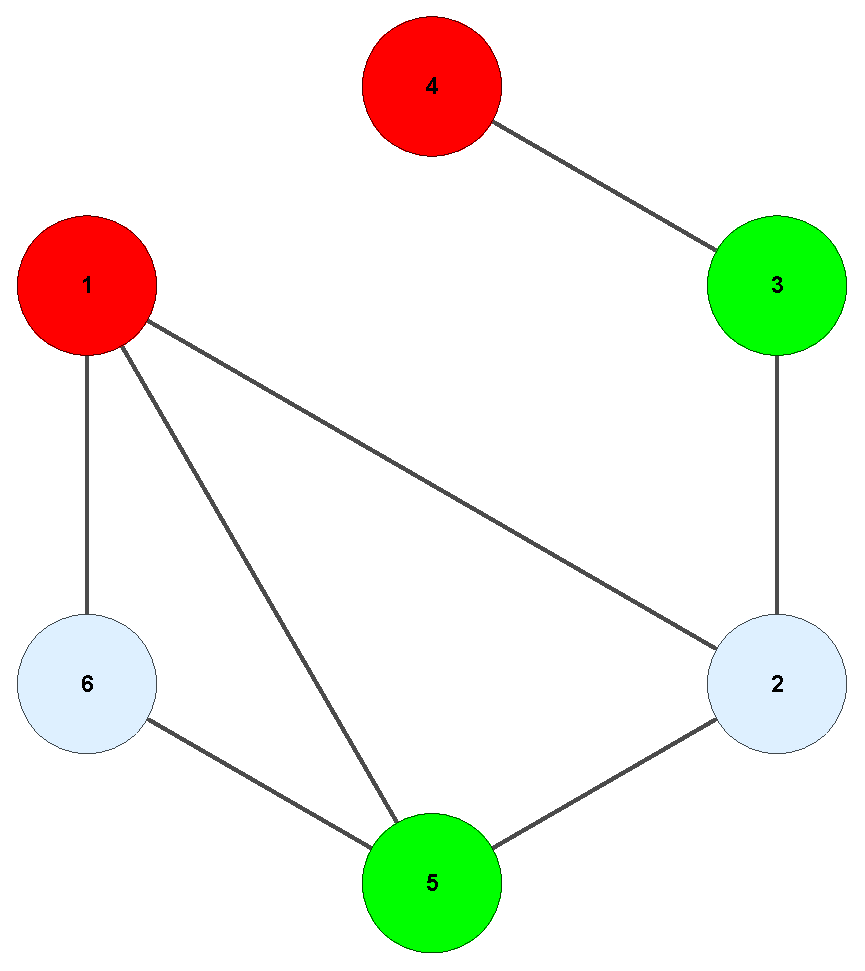
\includegraphics[scale=.4]{RFallocation3}}
  \end{center}
\end{figure}



}


\frame
{
  \frametitle{Alcuin's River Crossing Puzzle}


\begin{figure}[htp]
  \begin{center}
    \subfigure{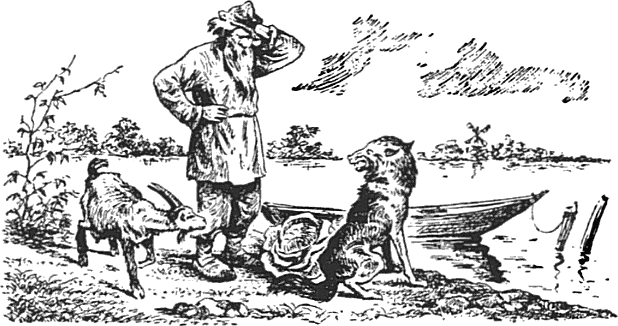
\includegraphics[scale=.3]{wgc.png}}
  \end{center}
\end{figure}

A traveler comes to a riverbank with a wolf, a goat, and a head of cabbage. There is a boat that he can use for crossing over to the other bank, but  it can carry no more than two, the traveler himself and one of other three. If left alone together, the goat will eat the cabbage and the wolf will eat the goat. The wolf does not eat cabbage. How does the traveler transport his animals and his cabbage to the other side intact in a minimum number of back-and-forth trips?

}

\frame
{
  \frametitle{Alcuin's River Crossing Activity}


\begin{figure}[htp]
  \begin{center}
    \subfigure{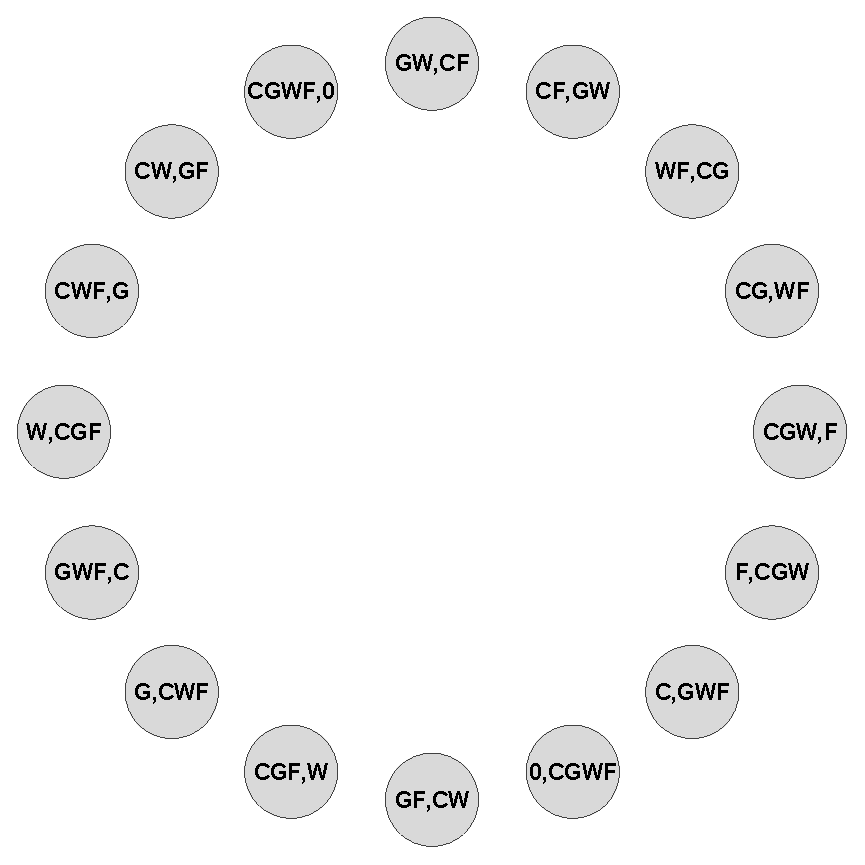
\includegraphics[scale=.5]{CGWFgraph1}}
  \end{center}
\end{figure}



}


\frame
{
  \frametitle{Alcuin's River Crossing Activity}


\begin{figure}[htp]
  \begin{center}
    \subfigure{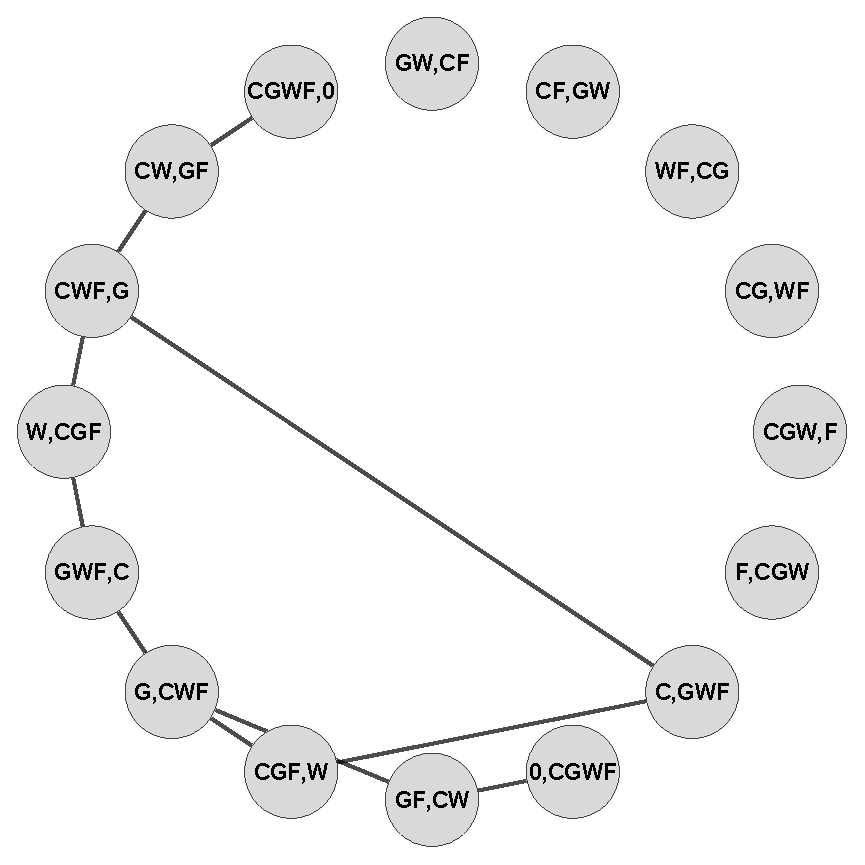
\includegraphics[scale=.5]{CGWFgraph2}}
  \end{center}
\end{figure}



}



\frame
{
  \frametitle{Important Definitions}

\begin{definition}[Graph]
A {\bf graph} is a pair $G=(V,E)$ with $E \subseteq V\times V$ where $V=V(G)$ is the set of vertices of $G$ and $E=E(G)$ is the set of edges of $G$
\end{definition}

\begin{definition}[Simple]
A graph is {\bf simple} if it contains no loops or multi-edges.
\end{definition}

\begin{definition}[Adjacent]
Two vertices $x$ and $y$ are {\bf adjacent} if $(x,y)$ is an element of  $E$.
\end{definition}


}

\frame
{
  \frametitle{Important Definitions}



\begin{definition}[Degree of a vertex]
The {\bf degree} of a vertex $x$ is $d(x)$ and is the number of vertices adjacent to $x$.
\end{definition}

\begin{definition}[Pedant vertex]
The {\bf pedant} or leaf  vertex is a vertex with degree 1.
\end{definition}


\begin{definition}[$n$-regular]
A graph is called {\bf $n$-regular} if every vertex in the graph has degree $n$.
\end{definition}




}





\frame
{
\frametitle{Definitions}
\begin{definition}[Walk]
A {\bf walk} in a graph is a sequence of vertices $v_1,v_2,\cdots,v_k$ where $(v_i, v_{i+1})$ is an edge for all $1 \leq i \leq k-1$. Its length is $k-1$. A walk is {\bf closed} if $v_1 = v_k$.
\end{definition}

\begin{definition}[Trail]
A {\bf trail} is a walk with no repeated edges.
\end{definition}

\begin{definition}[Path]
A {\bf path} is a trail with no repeated vertices, with the exception that the first and last vertex may be the same.
\end{definition}

\begin{definition}[Cycle]
A {\bf cycle} is a path with the first and last vertex the same.
\end{definition}

}

\frame
{
\frametitle{Definitions}

\begin{definition}[Subgraph]
A { \bf subgraph} of a graph $G$ is a graph $H$ with $V(H) \subseteq V(G)$
and $E(H) \subseteq E(G)$.
\end{definition}


\begin{definition}[Connected]
A graph is {\bf connected} if every pair of vertices is joined by a path.
\end{definition}

\begin{definition}[Component]
A maximally connected subgraph of a graph is a {\bf component}.
\end{definition}

\begin{definition}[Acyclic]
A graph is {\bf acyclic} if it has no cycles.
\end{definition}

}



\frame
{
  \frametitle{Degree sequence Activity}
  
\begin{definition}[Degree sequence of a graph]
The degree sequence of a graph is a graph with vertices
$v_1,\cdots,v_n$ is $d(v_1),\cdots,d(v_n)$ where degrees are listed in decreasing order.
\end{definition}
  

{\bf Degree Sequence activity}\\
1. Find graphs for the following degree sequences: (2,2,2),(2,2,2,2)(2,2,2,2,2)\\
2. Find graphs for the following degree sequences:(1,1),(2,2,2),(3,3,3,3)\\
3. Can you find graphs for the following degree sequences: (3,3,3,2) ,(3,3,2,2,1,1), (3,3,2,2,1)\\
4. Can you create a simple graph for any degree sequence?  What are the restrictions?


}


\frame
{
  \frametitle{More degree sequence activities}
For the following degree sequences: 
\vfill
(4,4,3,3,3,3)\\
(3,3,3,3,3)\\
(4,3,1,1,1,1,1)\\
(3,3,2,2,2,1,1,1,1) \\
\vfill
Can you construct: a connected graph? a disconnected graph? A graph where there is a cycle? A connected graph with a cycle?
If no, what goes wrong?


}


\frame
{
  \frametitle{Some algebraic constraints on simple graphs}

{\bf Question 1} What can you say about the pairity (odd or even) for the sum of degrees of a graph?  Can you write down a relationship between the sum of degress of a graph and the number of edges in a graph?

\vfill
{\bf Question 2} What is the maximum number of edges in a simple graph?
\vfill
\pause
{\bf Handshaking Lemma}  The sum of the degrees in a graph is equal to twice the number of edges.
\vfill
\vfill
{\bf Lemma} The maximum number of edges in a simple graph is $\binom{n}{2}$.

}






\end{document}

